\documentclass[border=4pt]{standalone}

\usepackage{pgfplots}
\usepackage{pgfplotstable}
\pgfplotsset{compat=1.18, width=8.5cm, height=5.6cm, tick label style={font=\small}, label style={font=\small}, legend cell align=left, legend style={font=\small, draw=none, fill=none}}

\definecolor{plnavy}{HTML}{1F4E89}
\definecolor{plrose}{HTML}{B85A52}
\definecolor{plsage}{HTML}{93CC9E}
\definecolor{plsand}{HTML}{E0BE78}
\definecolor{plplum}{HTML}{8E7BB5}
\definecolor{plgray}{HTML}{6E6E6E}

% ==== data: one \methodbar{position}{mean}{error}{color} per bar ====
\newcommand{\methodbars}{
  \methodbar{1}{0.538}{0.012}{plgray!40}
  \methodbar{2}{0.536}{0.027}{plsand!40}
  \methodbar{3}{0.545}{0.024}{plrose!30}
  \methodbar{4}{0.577}{0.021}{plrose!55}
  \methodbar{5}{0.767}{0.032}{plsand!70!black!70}
  \methodbar{6}{0.588}{0.018}{plsage!20}
  \methodbar{7}{0.684}{0.027}{plsage!40}
  \methodbar{8}{0.793}{0.024}{plsage!60}
  \methodbar{9}{0.842}{0.019}{plnavy!75}
}
\pgfplotsset{method names/.style={xtick={1,...,9}, xticklabels={B1,B2,B3,B4,B5,V1,V2,V3,Ours}}}

\newcommand{\methodbar}[4]{\addplot[fill=#4, draw=none, bar shift=0pt, error bars/.cd, y dir=both, y explicit, error bar style={black, line width=0.7pt}, error mark options={rotate=90, black, mark size=2.5pt, line width=0.7pt}] coordinates {(#1,#2) +- (0,#3)};}

\begin{document}
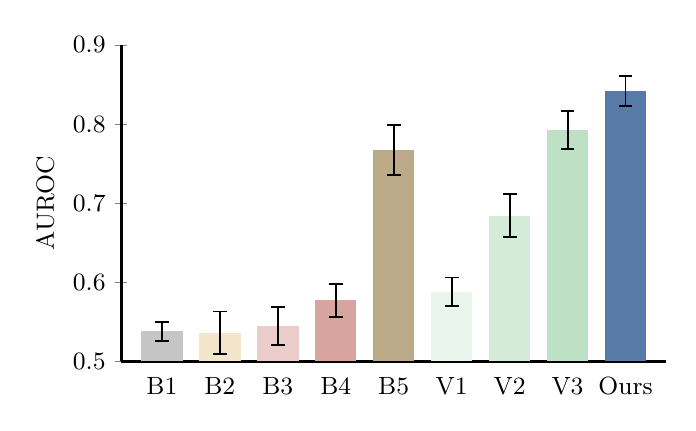
\begin{tikzpicture}
\begin{axis}[ybar, bar width=15pt, axis lines=left, axis line style={line width=1.2pt, -}, ymin=0.5, ymax=0.9, ytick={0.5,0.6,...,0.9}, xmin=0.3, xmax=9.7, xtick style={draw=none}, ylabel={AUROC}, method names, yticklabel style={/pgf/number format/fixed, /pgf/number format/precision=1, /pgf/number format/fixed zerofill}]
  \methodbars
\end{axis}
\end{tikzpicture}
\end{document}
